% !TEX TS-program = XeLaTeX
% !TEX spellcheck = en-US
\documentclass[aspectratio=169]{beamer}

\usetheme{example}

\title{Lecture 5:\\ Model Selection, Evaluation, and Assessment}
\institute{GRA4160: Predictive Modelling with Machine Learning}
\date{February 6th, 2025}
\author{Vegard H\o ghaug Larsen}

\begin{document}

\maketitle

\frame{
  \frametitle{Plan for Today}
  \begin{enumerate}
    \item Recap from Last Week
    \item Model Selection, Evaluation, and Assessment
    \item Information Criteria
    \item Cross-Validation
    \item Bias-Variance Trade-off
  \end{enumerate}
}

\begin{frame}
\frametitle{Recap: Logistic Regression}
\begin{itemize}
    \item \textbf{Purpose:} Binary classification (generalized to multi-class).
    \item \textbf{Log-odds Model:} 
    \[
      \log\Bigl(\frac{p}{1-p}\Bigr) = \beta_0 + \beta_1 x_1 + \cdots + \beta_k x_k.
    \]
    \item \textbf{Sigmoid Function:} Maps any real value to \([0,1]\) for valid probabilities:
    \[
      p = \frac{1}{1 + e^{-z}}.
    \]
    \item \textbf{Estimation:} 
      \begin{itemize}
        \item Fit via maximum likelihood (minimize negative log-likelihood).
        \item Interpret coefficients in terms of odds ratios (\(e^\beta\)).
      \end{itemize}
\end{itemize}
\end{frame}


\begin{frame}
\frametitle{Recap: Decision Trees}
\begin{itemize}
    \item \textbf{Decision Trees}
    \begin{itemize}
        \item Non-parametric, recursively splits data to purify classes.
        \item Splits chosen by impurity measures (Gini, Entropy).
        \item Advantages: Interpretability, no feature scaling needed.
        \item Drawbacks: Prone to overfitting if not pruned.
    \end{itemize}
\end{itemize}
\end{frame}


\frame{
  \frametitle{What is Model Selection?}
  \begin{itemize}
    \item Model selection is the process of choosing the best model from a set of candidate models.
    \item A common (but potentially risky) approach is to compare performance on a held-out \textbf{validation} set and select the model with the best score.
    \item \textbf{Pitfall:} Overusing a single validation set can lead to overfitting to that set.
    \item \textbf{Alternatives:}
      \begin{itemize}
        \item \textbf{Cross-validation} - averages performance over multiple folds.
        \item \textbf{Information criteria} - such as AIC or BIC, which balance model fit and complexity.
      \end{itemize}
  \end{itemize}
}

\frame{
  \frametitle{What is Model Evaluation?}
  \begin{itemize}
    \item Model evaluation measures how well a model performs on new, unseen data.
    \item Approaches include:
      \begin{itemize}
        \item Splitting data into training and testing sets.
        \item Using cross-validation techniques.
      \end{itemize}
    \item The aim is to estimate real-world performance.
    \item Common evaluation metrics include accuracy, precision, recall, ROC curves, and AUC.
    \item Visual tools like confusion matrices and decision boundary plots can help diagnose performance.
  \end{itemize}
}

\frame{
  \frametitle{Common Metrics for Model Evaluation}
  \begin{itemize}
    \item \textbf{Accuracy:} Fraction of all predictions that are correct.
    \item \textbf{Precision:} Fraction of positive predictions that are correct (important when false positives are costly).
    \item \textbf{Recall (Sensitivity):} Ability to capture all positive instances (crucial when false negatives matter).
    \item \textbf{ROC Curve:} Plots the true positive rate versus the false positive rate at different thresholds.
    \item \textbf{AUC:} The area under the ROC curve, providing an overall performance measure.
  \end{itemize}
  %\vspace{0.5em}
  %\small{(For more details, see Exercise 5 in the exercise notebook.)}
}

\frame{
  \frametitle{Understanding the Confusion Matrix}
  \begin{itemize}
    \item A confusion matrix summarizes a classification model’s performance.
    \item It is composed of:
      \begin{itemize}
        \item \textbf{True Positives (TP):} Correctly predicted positive instances.
        \item \textbf{True Negatives (TN):} Correctly predicted negative instances.
        \item \textbf{False Positives (FP):} Incorrectly predicted positives (Type I error).
        \item \textbf{False Negatives (FN):} Incorrectly predicted negatives (Type II error).
      \end{itemize}
    \item From these, we can compute:
      \begin{itemize}
        \item Precision = TP / (TP + FP)
        \item Recall = TP / (TP + FN)
        \item Accuracy = (TP + TN) / (TP + TN + FP + FN)
      \end{itemize}
    \item This matrix offers a fuller picture than accuracy alone.
  \end{itemize}
}

\frame{
  \frametitle{What is Model Assessment?}
  \begin{itemize}
    \item Model assessment goes beyond simple evaluation—it examines multiple facets of a trained model.
    \item Key aspects include:
      \begin{itemize}
        \item \textbf{Predictive Performance:} How well does the model generalize to new data?
        \item \textbf{Complexity:} How many parameters or how intricate is the model?
        \item \textbf{Interpretability:} How easy is it to understand the model’s decisions?
        \item \textbf{Computational Efficiency:} What are the resource requirements for training and prediction?
        \item \textbf{Scalability:} Can the model handle larger datasets or increased complexity?
      \end{itemize}
    \item Techniques like sensitivity analyses or stress tests can help ensure robustness.
    \item Cross-validation is central to assessing model generalizability.
  \end{itemize}
}

\frame{
  \frametitle{Introduction to Information Criteria}
  \begin{itemize}
    \item Information criteria are statistical tools that help balance model fit with model complexity.
    \item The goal is to select a model that explains the data well without being overly complex.
    \item Two commonly used criteria are:
      \begin{itemize}
        \item \textbf{Akaike Information Criterion (AIC)}
        \item \textbf{Bayesian Information Criterion (BIC)}
      \end{itemize}
    \item They rely on the concept of likelihood and penalize the number of parameters.
  \end{itemize}
}

\frame{
  \frametitle{Akaike and Bayesian Information Criteria}
  \begin{itemize}
    \item \textbf{Akaike Information Criterion (AIC):}
      \begin{itemize}
        \item Balances goodness of fit and complexity.
        \item A lower AIC indicates a better model.
        \item Calculated as: 
          \[
          AIC = 2k - 2\ln(L)
          \]
          where \( k \) is the number of parameters and \( L \) is the model likelihood.
      \end{itemize}
    \pause
    \item \textbf{Bayesian Information Criterion (BIC):}
      \begin{itemize}
        \item Similar in form to AIC, but applies a larger penalty for complexity.
        \item Tends to favor simpler models.
        \item Calculated as:
          \[
          BIC = \ln(n)k - 2\ln(L)
          \]
          where \( n \) is the sample size.
      \end{itemize}
    \pause
    \item \textbf{Note:} Both AIC and BIC are relative measures—use them to compare models on the same dataset.
  \end{itemize}
}

\frame{
  \frametitle{\(k\)-Fold Cross-Validation}
  \begin{itemize}
    \item The dataset is divided into \( k \) equal (or nearly equal) parts (folds).
    \item In each of \( k \) iterations:
      \begin{itemize}
        \item One fold is held out as the test set.
        \item The remaining \( k-1 \) folds form the training set.
      \end{itemize}
    \item Performance is averaged across all folds, reducing bias and variance in the estimate.
    \item Particularly useful when data is limited.
    \item Common choices for \( k \) are 5 or 10, though the best value depends on the dataset size and computational resources.
  \end{itemize}
}

\frame{
  \frametitle{\(k\)-Fold Cross-Validation}
  \begin{center}
    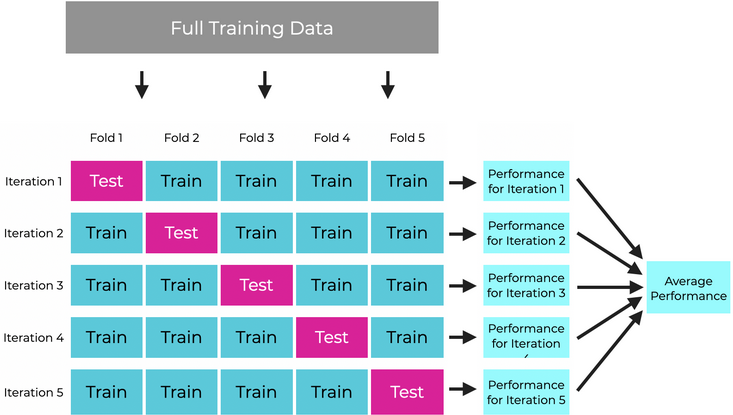
\includegraphics[scale=0.5]{figures/kFold_validation.png}
  \end{center}
  }


\frame{
  \frametitle{Additional Cross-Validation Techniques}
  \begin{itemize}
    \item \textbf{Stratified \(k\)-fold:} Ensures each fold maintains the same class distribution as the full dataset (especially useful for imbalanced classes).
    \item \textbf{Leave-One-Out Cross-Validation (LOOCV):} Uses all but one observation for training; although nearly unbiased, it can be computationally expensive.
    \item \textbf{Repeated Cross-Validation:} Repeats the \( k \)-fold process multiple times with different splits to obtain more robust performance estimates.
  \end{itemize}
}

\frame{
  \frametitle{The Bias-Variance Trade-off}
  \begin{itemize}
    \item A key concept in understanding model performance on unseen data.
    \item \textbf{Bias:}
      \begin{itemize}
        \item Error from overly simplistic assumptions.
        \item Leads to underfitting (missing important patterns).
      \end{itemize}
    \pause
    \item \textbf{Variance:}
      \begin{itemize}
        \item Error from sensitivity to small fluctuations in the training data.
        \item Leads to overfitting (capturing noise as if it were signal).
      \end{itemize}
    \pause
    \item The goal is to balance bias and variance to achieve a model that generalizes well.
  \end{itemize}
}

\frame{
  \frametitle{Managing Bias and Variance}
  \begin{itemize}
    \item \textbf{High Bias (Underfitting):}
      \begin{itemize}
        \item Remedies include increasing model complexity (more features or a more flexible algorithm) or reducing regularization.
      \end{itemize}
    \pause
    \item \textbf{High Variance (Overfitting):}
      \begin{itemize}
        \item Remedies include simplifying the model, increasing regularization, or gathering more training data.
      \end{itemize}
  \end{itemize}
}

\frame{
  \frametitle{Visualizing the Bias-Variance Trade-off}
  \begin{center}
    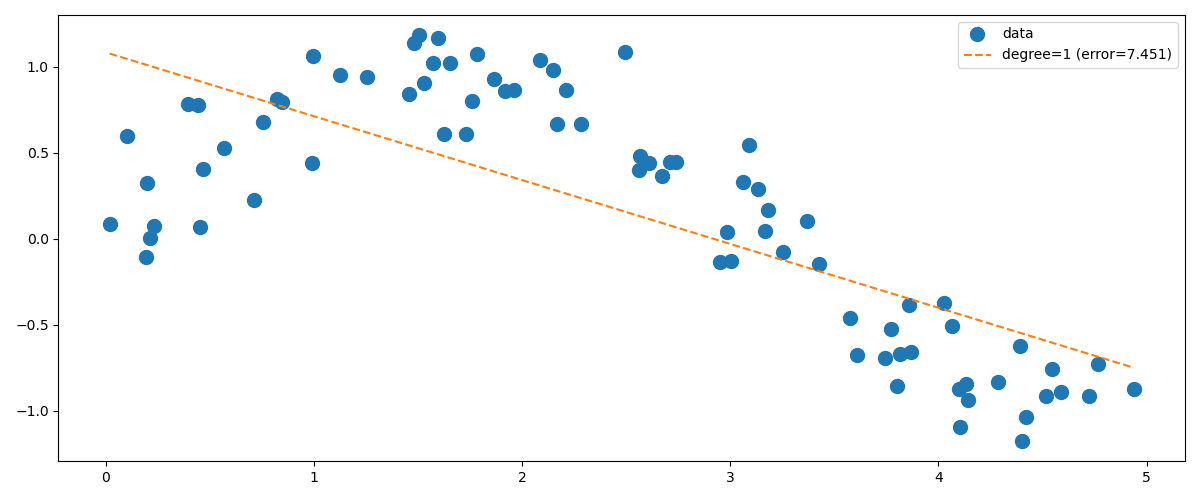
\includegraphics[scale=0.5]{figures/bias_variance_tradeoff_1.png}
    \vspace{0.5em}
    
    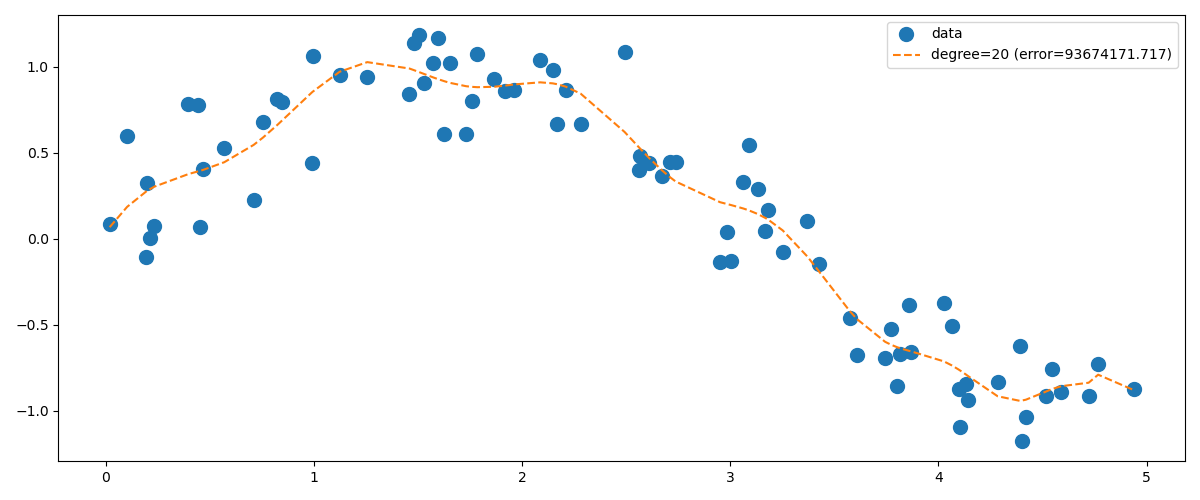
\includegraphics[scale=0.5]{figures/bias_variance_tradeoff_2.png}
    
    \small{(Left: Example of high bias/underfitting. Right: Example of high variance/overfitting.)}
  \end{center}
}

\frame{
  \frametitle{Summary and Key Takeaways}
  \begin{itemize}
    \item \textbf{Model Selection:} Use techniques such as cross-validation and information criteria (AIC/BIC) to balance model fit and complexity.
    \item \textbf{Model Evaluation:} Assess performance using metrics (accuracy, precision, recall, AUC) and diagnostic tools (confusion matrix).
    \item \textbf{Model Assessment:} Consider broader factors like interpretability, computational efficiency, and scalability.
    \item \textbf{Cross-Validation:} Essential for obtaining robust performance estimates, especially when data is scarce.
    \item \textbf{Bias-Variance Trade-off:} Strive for a balance to avoid underfitting (high bias) and overfitting (high variance).
  \end{itemize}
}

% \frame{
%   \frametitle{Questions?}
%   \begin{center}
%     \Large{Any questions or points for discussion?}
%   \end{center}
% }

\end{document}
